\documentclass{beamer}
\mode<presentation>
\usepackage{tikz}
\setbeamertemplate{caption}{\insertcaption}
\renewcommand{\thefootnote}{\fnsymbol{footnote}}
% \usepackage{pdfpc-movie}
\usepackage{graphicx} %The mode "LaTeX => PDF" allows the following formats: .jpg  .png  .pdf  .mps
% \usepackage{media9}
\usetikzlibrary{lindenmayersystems,shapes.geometric,positioning,math,calc}
\title{Fractals}
\author[dishajk]{Disha Kuzhively}
\institute{International Centre for Theoretical Sciences - TIFR, Bangalore}
\date[SGB]{7 March 2026}

\pgfdeclarelindenmayersystem{Koch curve}{\rule{F -> F+F--F+F}}

\pgfdeclarelindenmayersystem{Cantor set}{
    \rule{F -> FfF}
    \rule{f -> fff}
}
\pgfdeclarelindenmayersystem{Sierpinski Gasket}{
\symbol{X}{\pgflsystemdrawforward}
\symbol{A}{\pgflsystemdrawforward}
\symbol{+}{\pgflsystemturnright} % Explicitly define + and - symbols.
\symbol{-}{\pgflsystemturnleft}
\rule{A -> A-X+A+X-A}
\rule{X -> XX}
}
\pgfdeclarelindenmayersystem{Dragon curve}{
\symbol{X}{\pgflsystemdrawforward}
\symbol{A}{\pgflsystemdrawforward}
\symbol{+}{\pgflsystemturnright} % Explicitly define + and - symbols.
\symbol{-}{\pgflsystemturnleft}
\rule{A -> A+X}
\rule{X -> A-X}
}
\pgfdeclarelindenmayersystem{Penrose}{
\symbol{F}{\pgflsystemdrawforward}
\symbol{+}{\pgflsystemturnright} % Explicitly define + and - symbols.
\symbol{-}{\pgflsystemturnleft}
\rule{W -> YF++ZF----XF[-YF----WF]++}
\rule{X -> +YF--ZF[---WF--XF]+}
\rule{Y -> -WF++XF[+++YF++ZF]-}
\rule{Z -> --YF++++WF[+ZF++++XF]--XF}
}
\tikzset{pics/monotile/.style args={a=#1,b=#2}{
  code={
    \def\a{#1}
    \def\b{#2}
  \filldraw[draw=green!50!blue, fill=red!50!white, thick] (0,0) --++(-90:{\a*\w})--++(0:{\b*\w})--++(-60:{\b*\w})--++(30:{\a*\w})--++(90:{2*\a*\w})--++(150:{\w*\a})--++(60:{\w*\b})--++(120:{\w*\b})--++(-150:{\w*\a})--++(-90:{\w*\a})--++(180:{\w*\b})--++(-120:{\w*\b})--cycle;
  }
}
}
\begin{document}
\begin{frame}
    \titlepage
\end{frame}
\begin{frame}
    \frametitle{Outline}
    \tableofcontents[pausesections]
    \end{frame}
\section{Fractals Around Us}
\begin{frame}
  \frametitle{Russian Dolls, Ferns, Trees, Cauliflower}
  \centering
  \only<1>{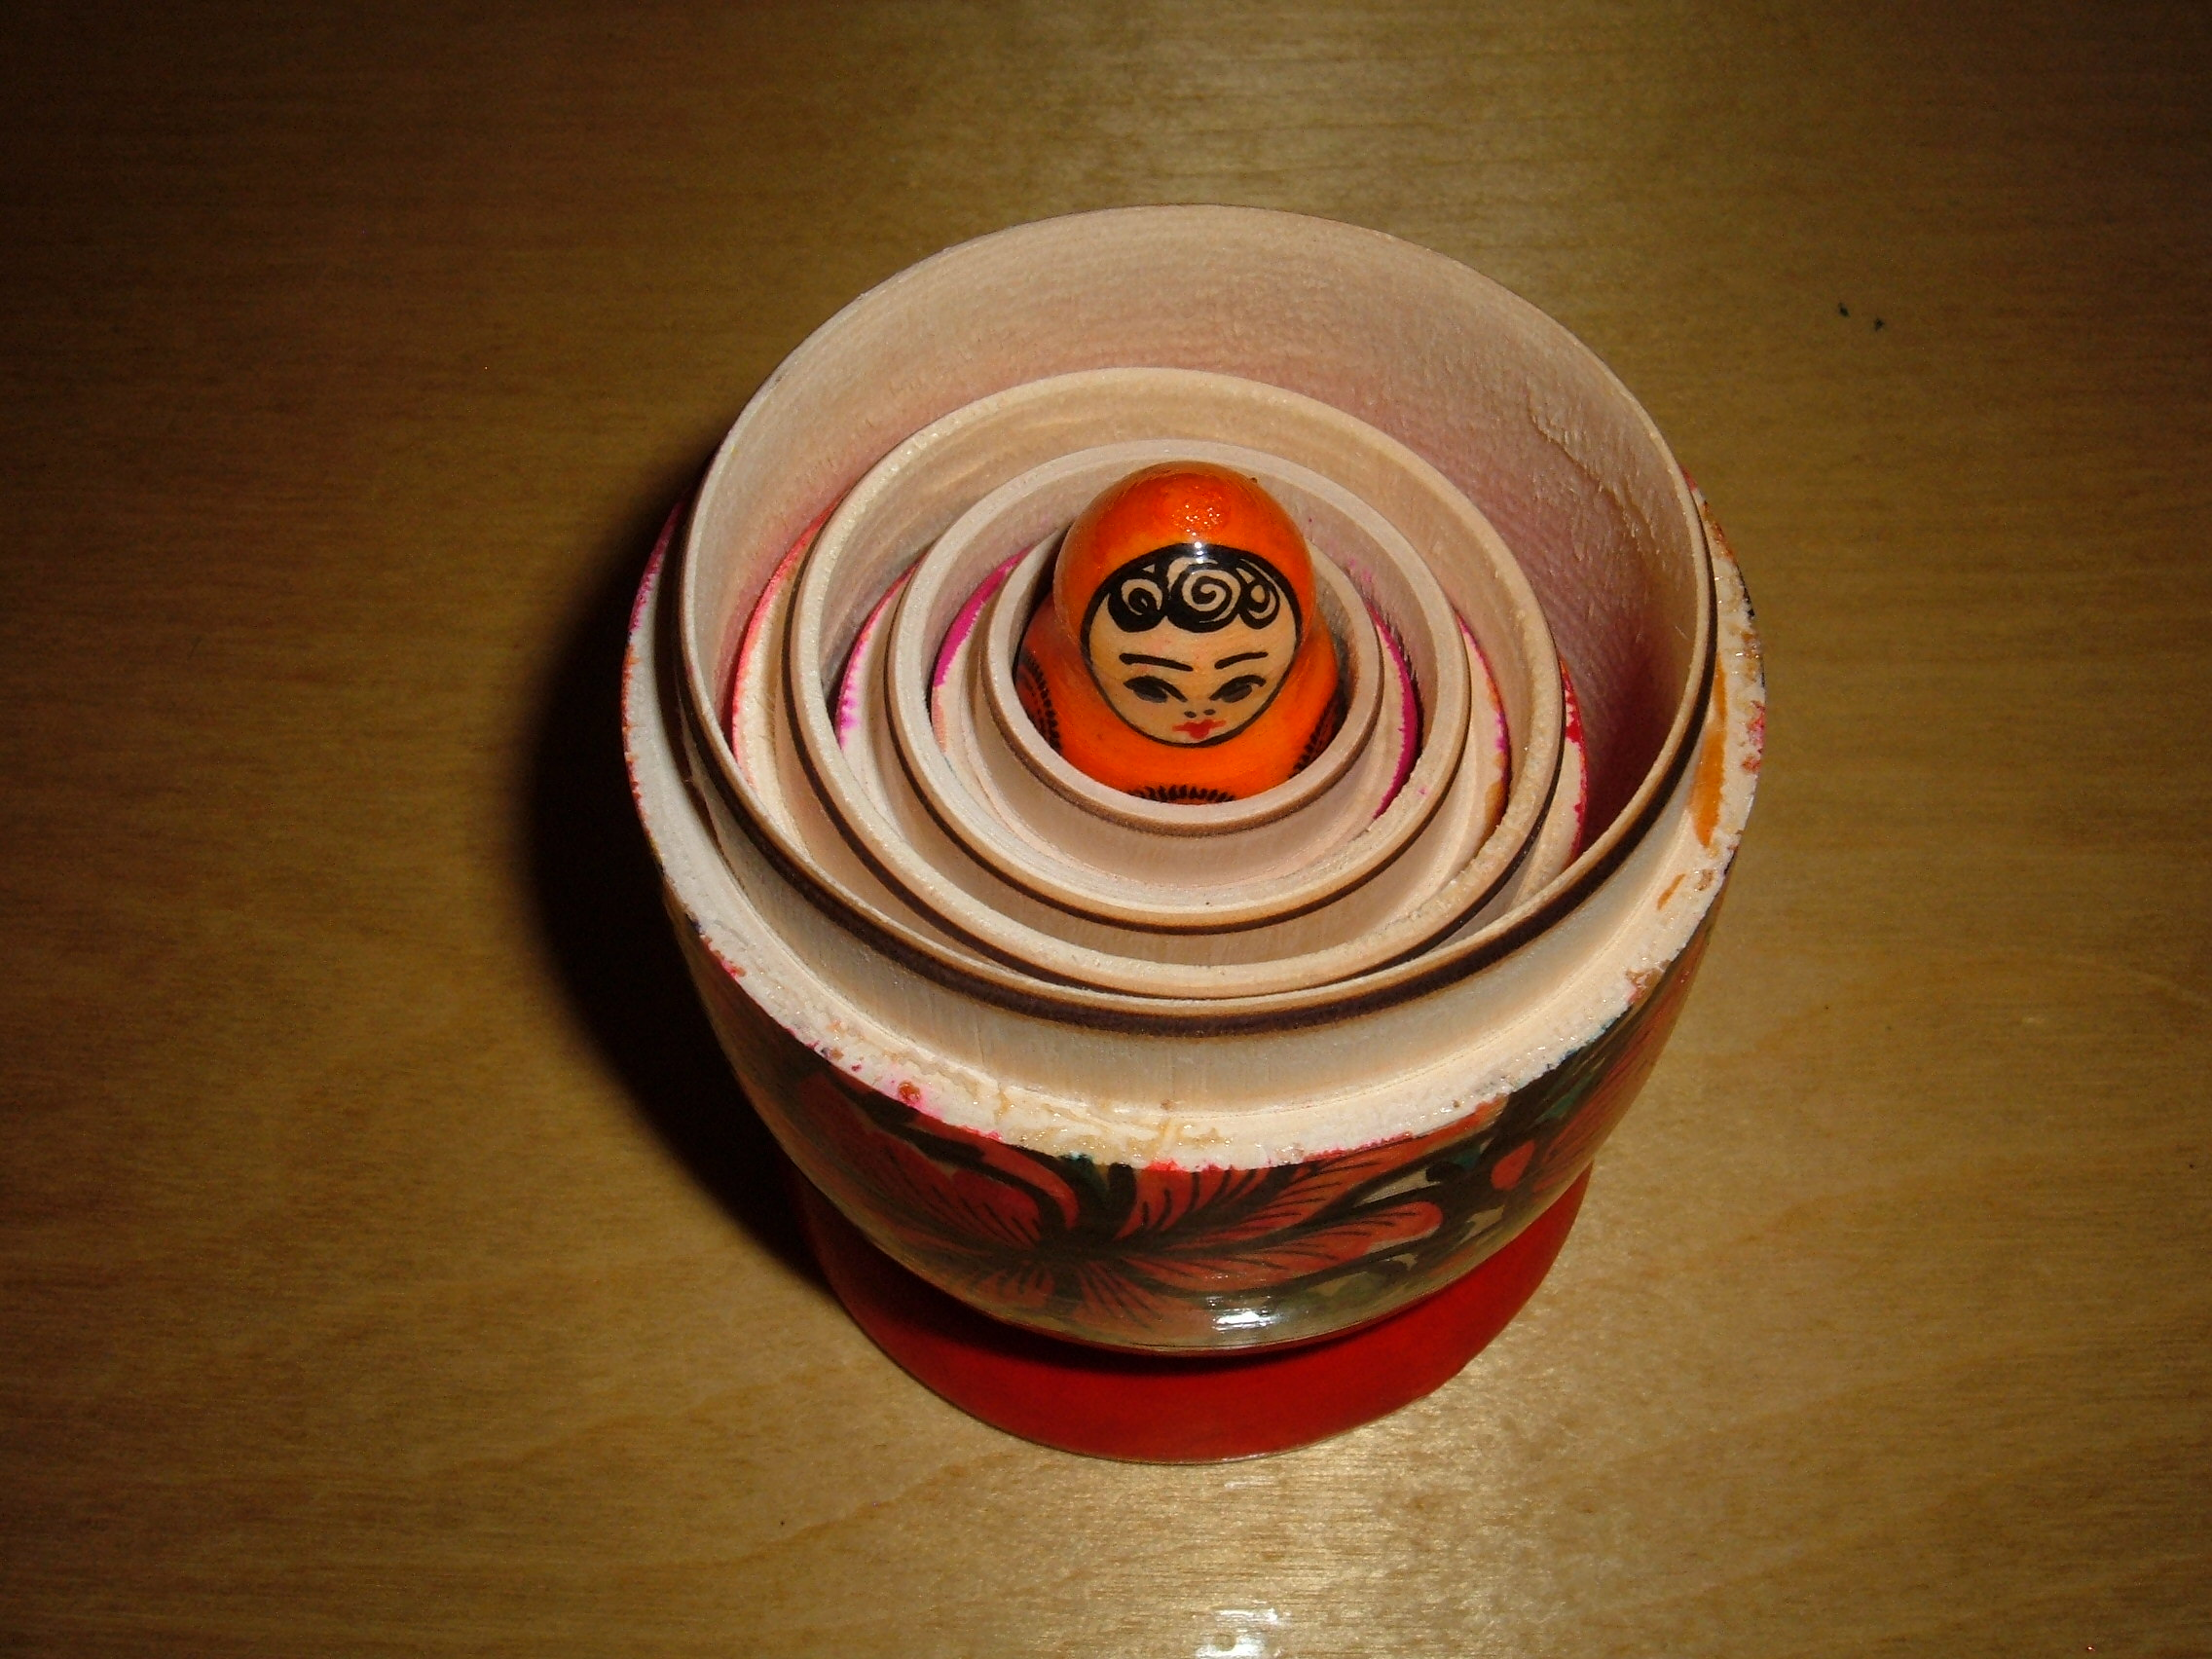
\includegraphics[height=0.5\textheight]{russiandolls}}
  \only<2>{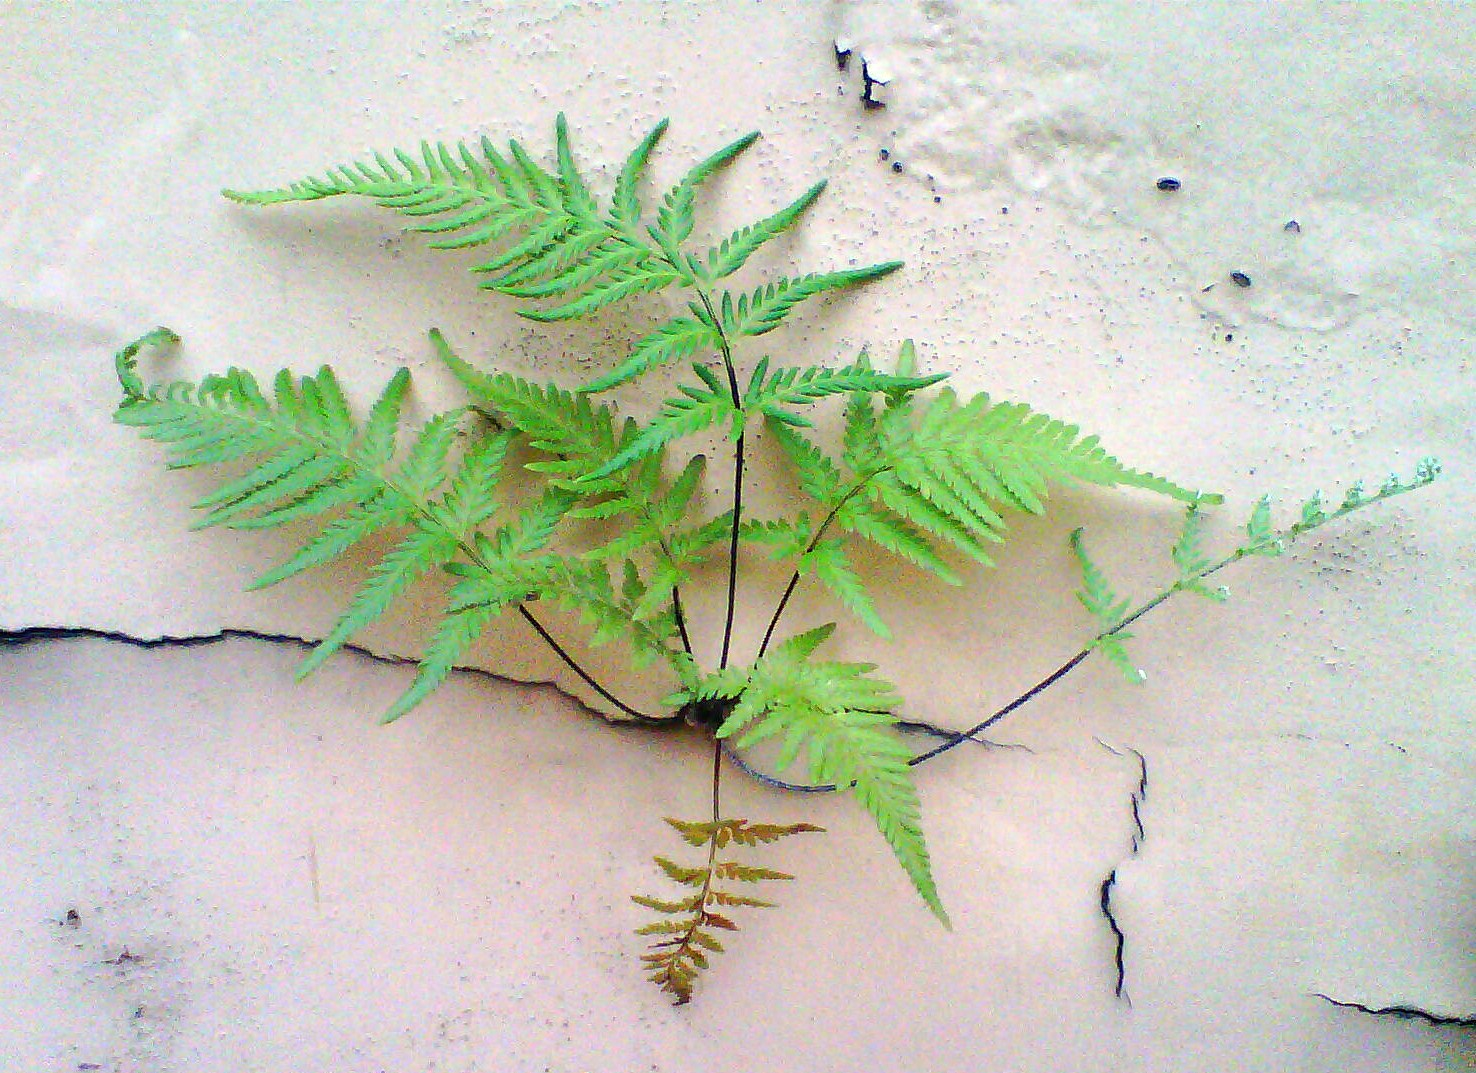
\includegraphics[height=0.5\textheight]{fern}\footnote{By Jml3 - Own work, \href{https://commons.wikimedia.org/w/index.php?curid=17823361}{CC BY-SA 3.0}}}
\end{frame}
\section{Fractals in Geometry}
\begin{frame}
  \frametitle{Koch curve}
  \centering
  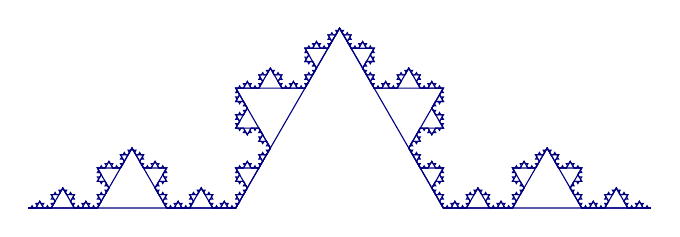
\begin{tikzpicture}
\foreach \i in {1,2,...,5}{
\only<\i>{
\draw [blue!50!black]
[l-system={Koch curve, step=225pt/3^\i, angle=60, axiom=F, order=\i}]
lindenmayer system;}}
\end{tikzpicture}
\end{frame}
\begin{frame}
  \frametitle{Cantor Set}
  \centering
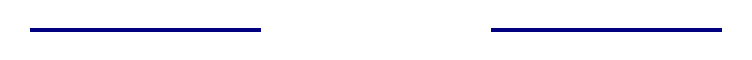
\begin{tikzpicture}
\foreach \i in {1,...,6}{\only<\i>{\draw [blue!50!black, ultra thick]
[l-system={Cantor set, step=250pt/3^\i, angle=0, axiom=F, order=\i}]
lindenmayer system;}}
\end{tikzpicture} 
\end{frame}
\begin{frame}
  \frametitle{Sierpinski Gasket}
  \centering
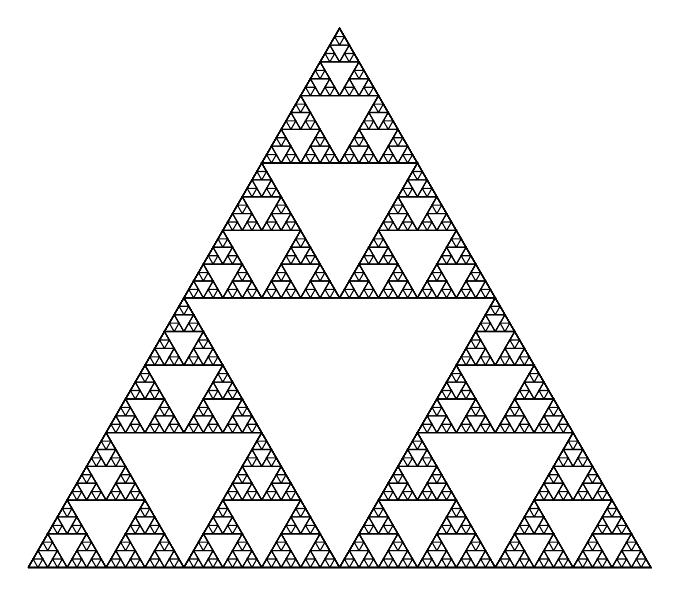
\begin{tikzpicture}
  \foreach \i in {1,...,6}{
    \only<\i>{
      \draw[lindenmayer system={Sierpinski Gasket, step=225pt/2^\i, axiom=A-X-X, order=\i, angle=120}] lindenmayer system;
    }
  }  
\end{tikzpicture} 
\end{frame}

\begin{frame}
  \frametitle{Dragon Curve}
  \centering
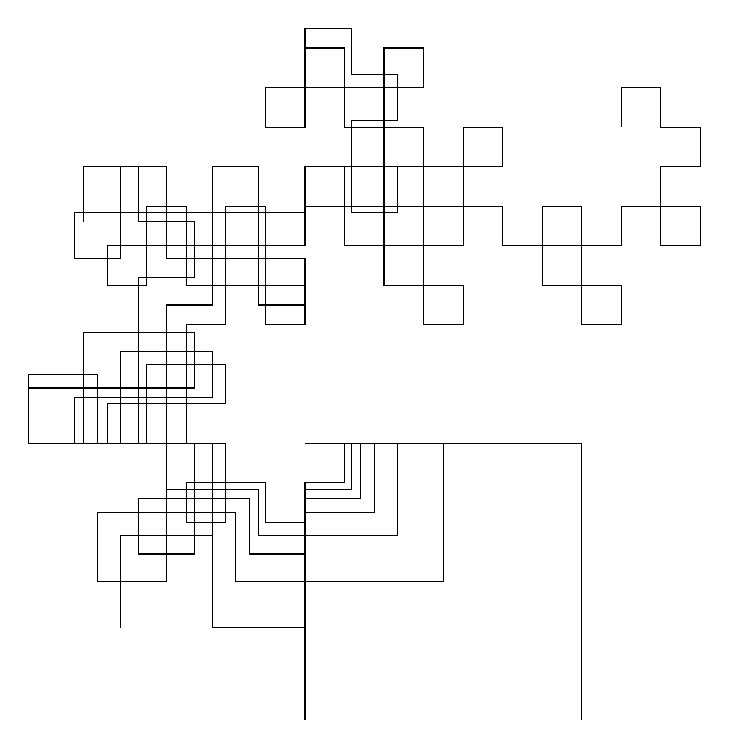
\begin{tikzpicture}
  \foreach \i in {1,...,7}{
    \only<\i>{
      \draw[lindenmayer system={Dragon curve, step=100pt/\i, axiom=A, order=\i, angle=90}] lindenmayer system;
    }
  }  
\end{tikzpicture} 
\end{frame}
\begin{frame}
  \frametitle{Penrose Tiling}
  \centering
  \foreach \i in {0,...,7}{
    \only<\i>{
      \includegraphics[width=0.9\textwidth]{penrose\i}
    }
  }  
\end{frame}
\begin{frame}
  \frametitle{Einstein}
\centering
\begin{tikzpicture}
\def\w{1}
\only<1>{\pic[rotate=90] at (0,0) {monotile={a=1,b=sqrt(3)}} node[below,yshift=-1cm] {Hat polykite};}
\only<3>{\pic[rotate=90] at (0,0) {monotile={a=1,b=sqrt(3)}} node[below,yshift=-1cm] {Tile(1,$\sqrt{3}$)};}
\only<4>{\pic[rotate=90] at (0,0) {monotile={a=1,b=0}} node[below,yshift=-1cm] {Tile(1,0), Comet};}
\only<5>{\pic[rotate=90] at (0,0) {monotile={a=0,b=1}} node[below,yshift=-1cm] {Tile(0,1), Chevron};}
\only<6>{\pic[rotate=90] at (0,0) {monotile={a=1,b=1}} node[below,yshift=-1cm] {Tile(1,1)};}

\end{tikzpicture}
\only<2>{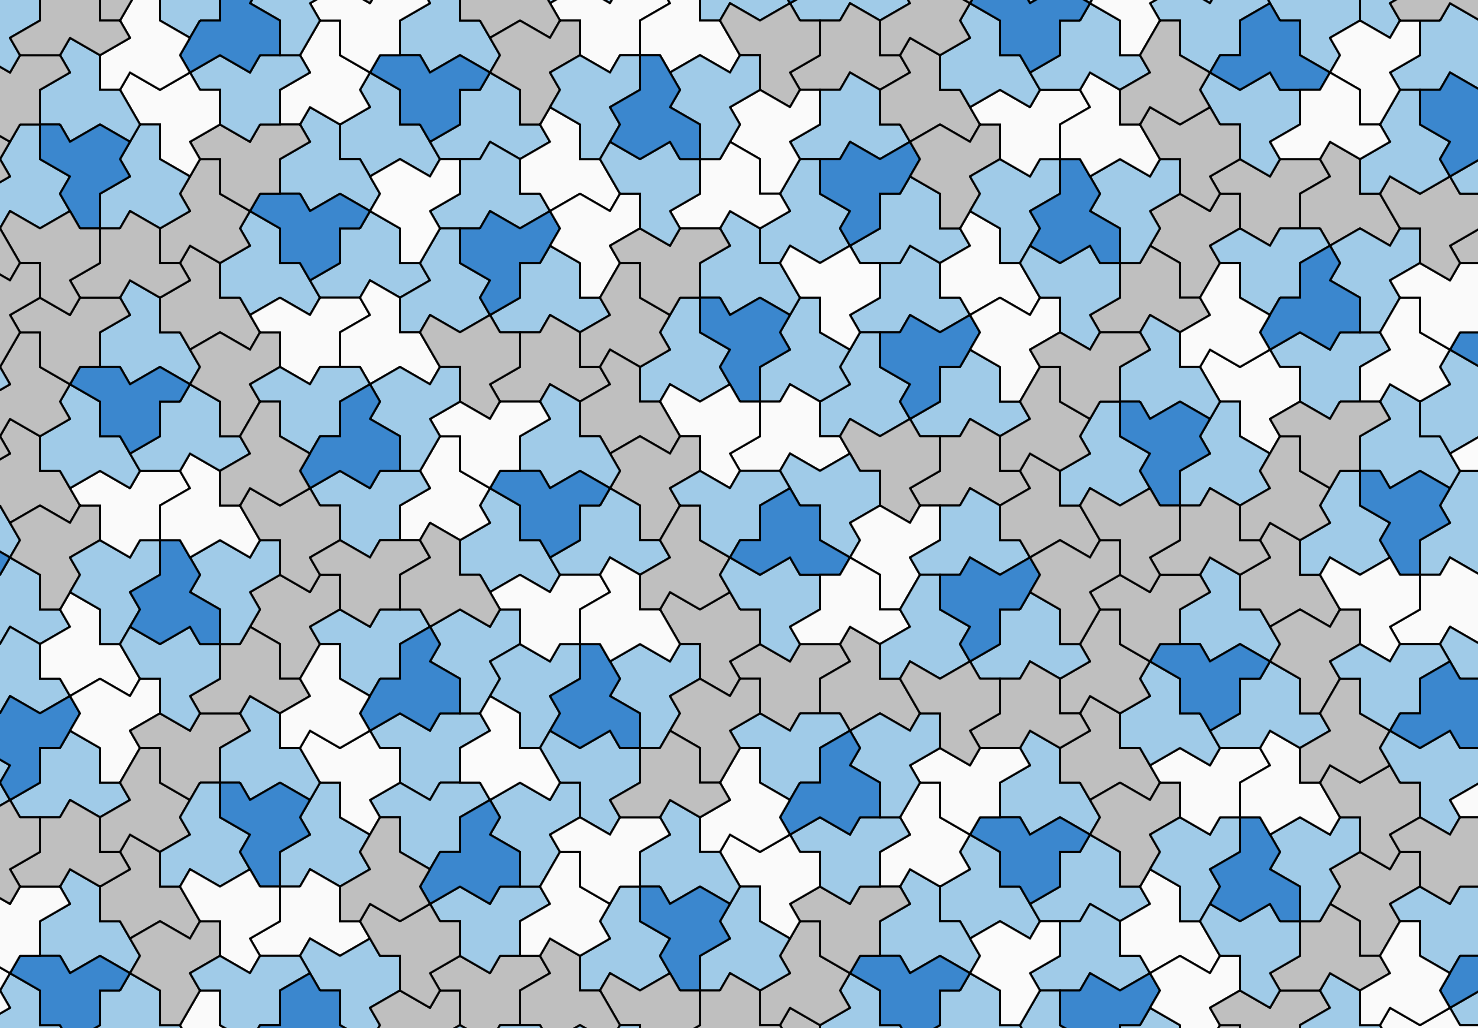
\includegraphics[width=0.9\textwidth]{hat}}
\end{frame}
\begin{frame}
  \frametitle{Spectre}
\begin{columns}
  \begin{column}{0.3\textwidth}
  \centering
  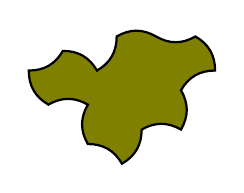
\begin{tikzpicture}[rotate=90]
    \pgfmathsetmacro{\w}{0.5}	%scale
	\pgfmathsetmacro{\a}{1}
	\pgfmathsetmacro{\b}{1}

    \coordinate (A) at (0,0);
    \coordinate (A2) at ($(A) + (-90:\a*\w)$);
    \coordinate (A3) at ($(A2) + (0:\b*\w)$);
    \coordinate (A4) at ($(A3) + (-60:\b*\w)$);
    \coordinate (A5) at ($(A4) + (30:\a*\w)$);
    \coordinate (A6) at ($(A5) + (90:\a*\w)$);
    \coordinate (A7) at ($(A6) + (90:\a*\w)$);
    \coordinate (A8) at ($(A7) + (150:\a*\w)$);
    \coordinate (A9) at ($(A8) + (60:\b*\w)$);
    \coordinate (A10) at ($(A9) + (120:\b*\w)$);
    \coordinate (A11) at ($(A10) + (-150:\a*\w)$);
    \coordinate (A12) at ($(A11) + (-90:\a*\w)$);
    \coordinate (A13) at ($(A12) + (180:\b*\w)$);
    \coordinate (A14) at ($(A13) + (-120:\b*\w)$);

    \tikzset{
        monotile/.pic={
            \draw[draw=black, thick,fill=green!50!red] (A) to[bend left] (A2) to[bend right] (A3) to[bend left] (A4) to[bend right] (A5) to[bend left] (A6) to[bend right] (A7) to[bend left] (A8)to[bend right] (A9) to[bend left] (A10) to[bend right] (A11) to[bend left] (A12)to[bend right] (A13) to[bend left] (A14) to[bend right] (A);
        }
    };
	\pic at (0,0) {monotile};
\end{tikzpicture}
  \end{column}
    \begin{column}{0.6\textwidth}
      \only<2>{
  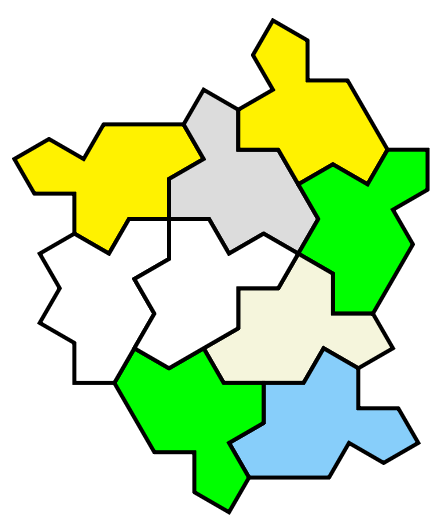
\includegraphics[width=0.7\textwidth]{supertile9}
}
  \end{column}
\end{columns}
\end{frame}
\begin{frame}
  \frametitle{Spectre}
\begin{columns}
    \begin{column}{0.3\textwidth}
  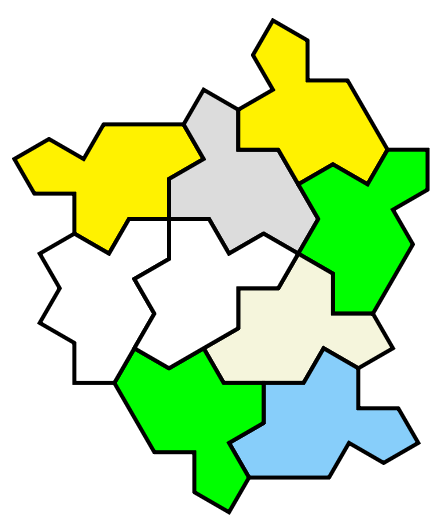
\includegraphics[width=0.9\textwidth]{supertile9}
  \end{column}
  \begin{column}{0.6\textwidth}
    \only<2>{
      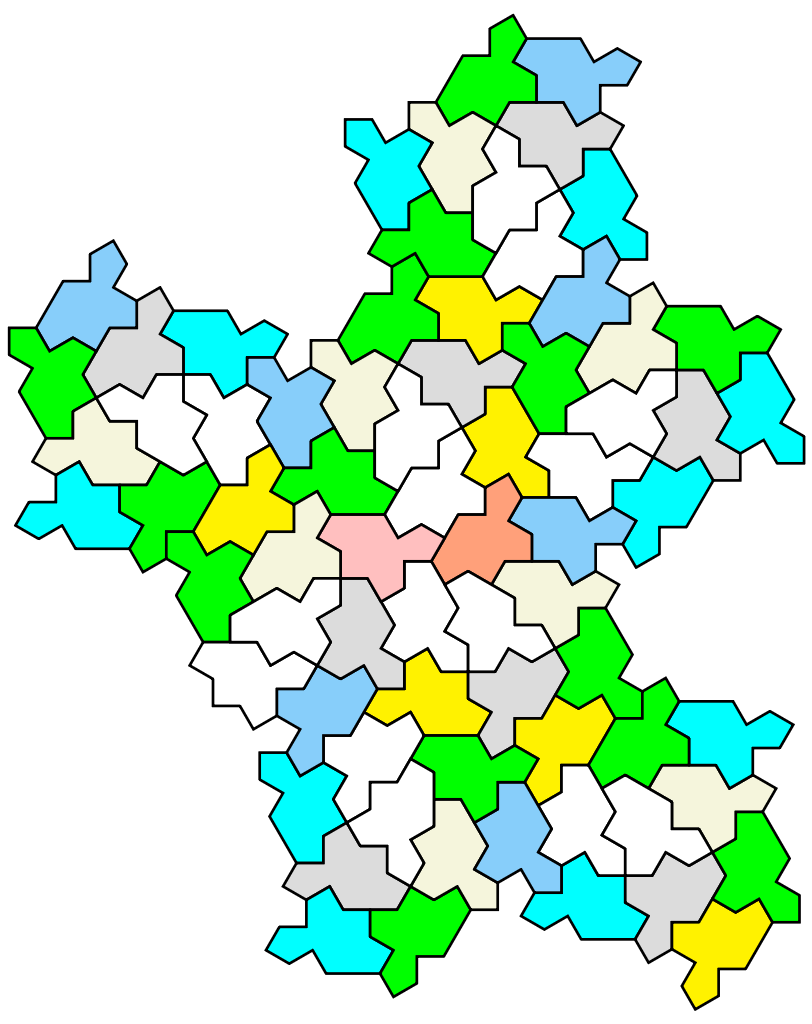
\includegraphics[width=0.9\textwidth]{supertile81}
    }
  \end{column}
\end{columns}
\end{frame}
\begin{frame}
  \frametitle{Spectre}

  \begin{columns}
  \begin{column}{0.3\textwidth}
      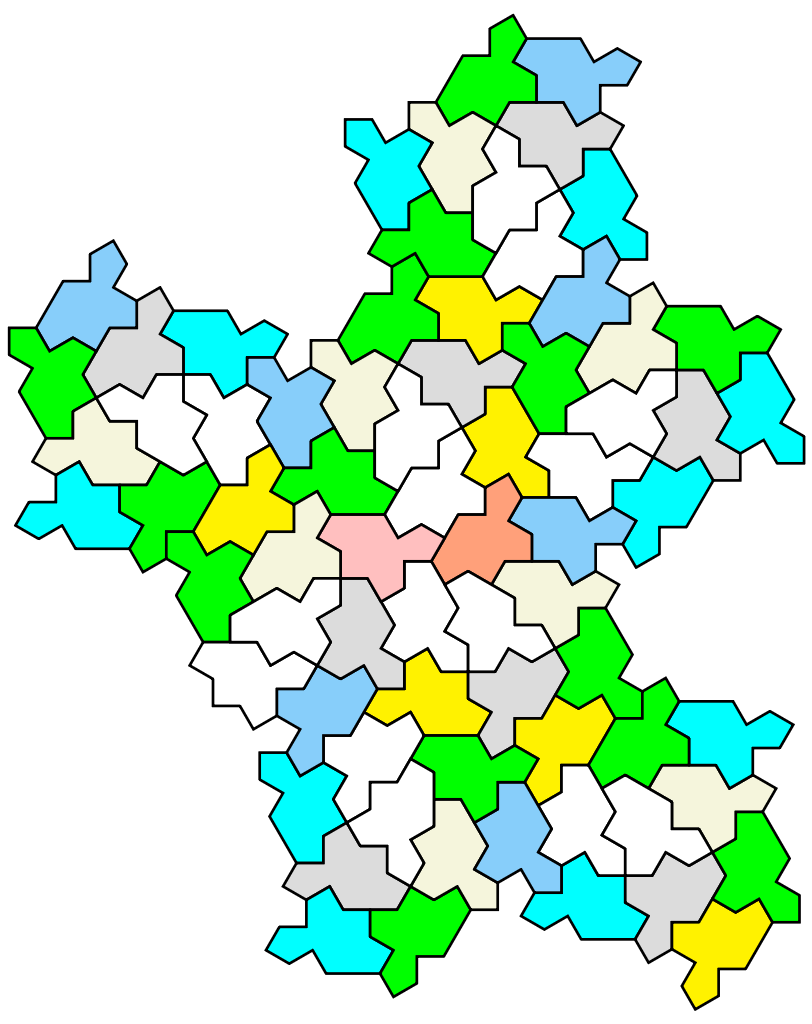
\includegraphics[width=0.9\textwidth]{supertile81}
  \end{column}
      \begin{column}{0.6\textwidth}
  \only<2>{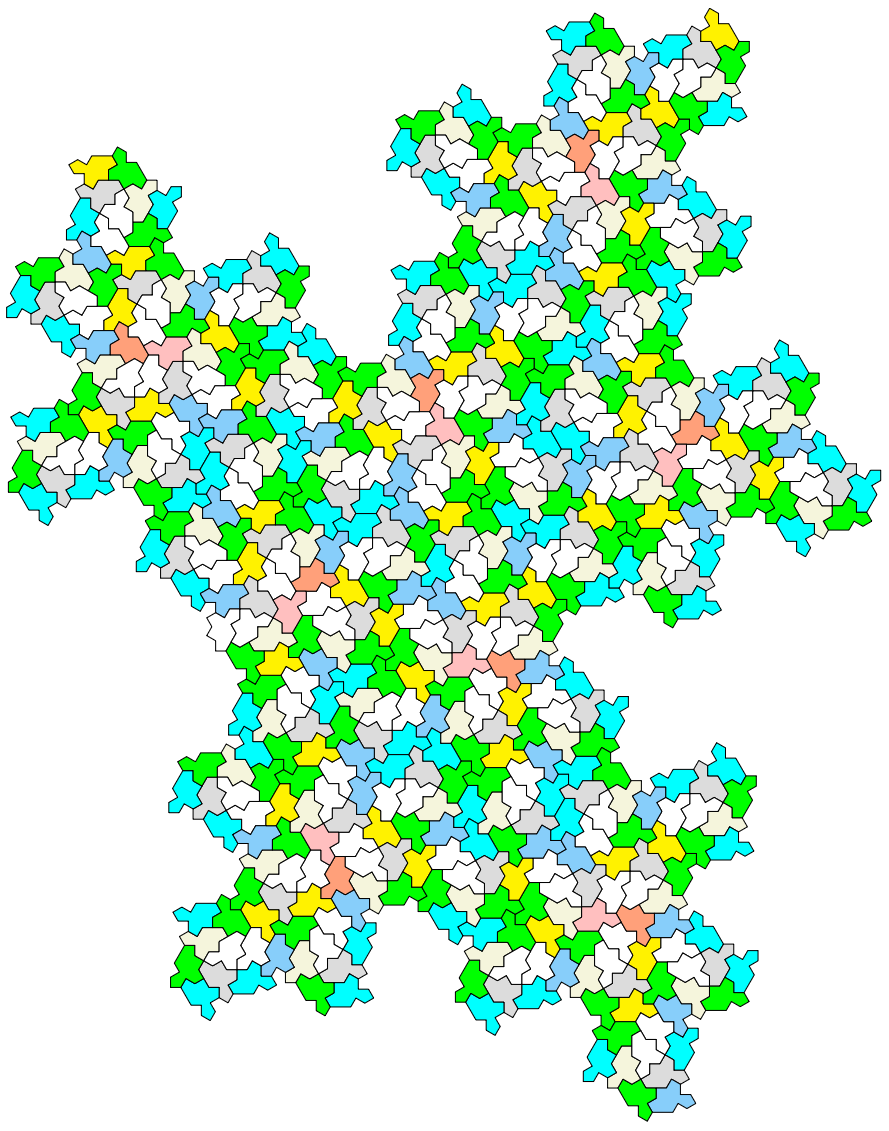
\includegraphics[width=0.9\textwidth]{supertile729}}
  \end{column}
\end{columns}
\end{frame}
\begin{frame}
\frametitle{Substitution Rules for Spectre}
	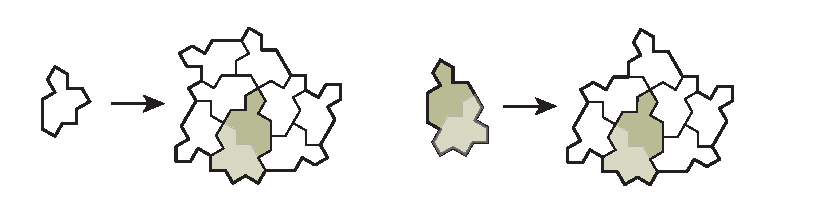
\includegraphics[width=\textwidth]{spectre_subrule.pdf}\footnote{Smith, D., Myers, J.S., Kaplan, C.S. and Goodman-Strauss, C., 2023. \emph{\href{https://doi.org/10.48550/arXiv.2305.17743}{A chiral aperiodic monotile}}. arXiv preprint arXiv:2305.17743}

  Replaces the Spectre by a cluster containing a Mystic and seven Spectres. 
  
  Replaces a Mystic by a cluster containing a Mystic and six Spectres
\end{frame}
\begin{frame}
\frametitle{References}
\begin{enumerate}
  \item[Book 1.]{\emph{The Fractal Geometry of Nature}, Beno\^{i}t Mandelbrot}
  \item[Article 2.]{\emph{\href{https://www.ams.org/publicoutreach/feature-column/fcarc-ribbons}{Penrose Tilings Tied up in Ribbons}}, David Austin}
  \item[Article 3.]{Smith, D., Myers, J.S., Kaplan, C.S. and Goodman-Strauss, C., 2023. \emph{\href{https://doi.org/10.48550/arXiv.2303.10798}{An aperiodic monotile}}. arXiv preprint arXiv:2303.10798.}
  \item[Article 4.]{Smith, D., Myers, J.S., Kaplan, C.S. and Goodman-Strauss, C., 2023. \emph{\href{https://doi.org/10.48550/arXiv.2305.17743}{A chiral aperiodic monotile}}. arXiv preprint arXiv:2305.17743}
\end{enumerate}
\end{frame}
\end{document}
  \begin{tikzpicture}
    \draw (0,0) rectangle (1,1) rectangle (0,2) rectangle (-2,0) rectangle (1,-3) rectangle (6,2);
  \end{tikzpicture}